% !Mode:: "TeX:UTF-8"
\chapter{绪论}

\section{研究背景}

\subsection{博物馆导览场景的数字化转型}
在国家文化数字化战略的顶层部署下，公共文化服务正从“文化资源数字化存储”走向“面向公众的数字化服务供给体系”建设\footnote{《中共中央办公厅、国务院办公厅关于推进实施国家文化数字化战略的意见》，中共中央办公厅、国务院办公厅印发，2022年。}。博物馆作为公共文化服务的重要触点，其导览服务也在这一转型中从静态说明牌、线性语音讲解逐步演进为更具交互性与个体适配能力的数字化体验形态。与此同时，数字文化产业相关政策强调以数字技术创新文化消费场景、发展线上线下一体化的新型文化体验\footnote{《文化和旅游部关于推动数字文化产业高质量发展的意见》，文化和旅游部印发，2020年。}，这进一步推动博物馆导览从内容科普走向交互导览的体验升级。

博物馆学习并非对展签或讲解文本的被动接收，而是观众在具体参观情境中围绕空间、对象与问题持续建构意义的过程\cite{falk2016,li2024,luo2024}。从当前数字导览实践看，语音讲解器、图文导览与脚本化数字讲解仍是主流形态，它们在内容标准化、规模化部署与运维稳定性方面具有现实优势，但也呈现出与博物馆学习机制不匹配的结构性局限：在交互层面，系统多停留于单轮问答与知识检索，难以维持跨轮次的探索式提问引导与主题推进\cite{duguleana2020,spiliotopoulos2020,varitimiadis2021}；在情境层面，系统对“当前展品—当前位置—当前参观阶段—当前关注点”的联动维护不足，易出现讲解与现场脱节、路径与理解不同步等问题\cite{hulusic2023,chin2023,tsitseklis2023}；在表达层面，语言内容与动作、视线、节奏等多模态线索缺乏一致性约束，导致观众虽“听到信息”却难形成稳定的注意力跟随与意义深化\cite{noh2021,cantucci2022,vanderheiden2022}。因此，博物馆数字化转型的关键难点不在更加充分地显示知识，而在面向博物馆导览的对话式数字人展示是否能够持续支持观众博物馆学习的过程。

面向人工智能时代的博物馆导览发展，本文围绕面向博物馆导览的对话式数字人展示展开研究，目标正是回应这一时代命题：通过将对话组织、情境理解与具身表达协同起来，提升观众在真实参观过程中的理解连续性、参与主动性与引导可感知性。相关研究结论不仅可为对话式数字人展示设计提供可验证的方法基础，也可为国家文化数字化战略与文博科技创新目标在一线公共文化服务中的落地提供实践支撑。

\subsection{生成式人工智能与数字人技术的应用契机}
文化与科技深度融合已被明确作为推动文化事业与文化产业高质量发展的重要方向\footnote{《关于促进文化和科技深度融合的指导意见》，科技部、中央宣传部、中央网信办、财政部、文化和旅游部、广播电视总局印发，2019年。}。在此背景下，大模型、语音识别与合成、数字人驱动等技术的快速发展，使博物馆导览从信息呈现走向交互服务具备了可落地的技术条件。生成式人工智能在语义理解与多轮生成方面的能力提升，使相关展示能够围绕观众的即时提问组织讲解内容、延展主题并进行解释性回应，从而更好适配参观过程中不断变化的认知需求。数字人作为具身交互媒介，能够把导览员在现场常用的引导线索外化为可被设计与调控的表达要素，包括语音语调与节奏控制、视线与指向、动作姿态与停顿提示等。这些非语言线索与讲解内容同步呈现，有助于观众更快定位展品对象、建立注意力焦点、理解讲解的组织结构，降低开放场域中跟随与理解的负担。数字人还能够通过持续的互动接续维持参观动机，在不同观众的知识基础与兴趣差异下提供更可持续的陪伴式导览体验。与此同时，对话式数字人展示在博物馆导览中的应用具备可复制与可扩展的服务特性，能够在导览员供给有限、客流波动明显的情境中提供相对一致的体验支持，契合公共文化服务数字化升级对稳定供给与普惠性的需求。

近年来，国内外已有博物馆开始引入面向导览的数字人展示或对话式模型用于观众服务与展览传播，例如在大型展览中推出面向观众的导览数字人，提供基础问答与讲解服务\footnote{《博物馆AI数字人导览：开启智能化服务新征程》，中国新闻网发布，2024年。}；也有文博机构推出面向公众传播的数字代言人，探索以虚拟形象承载文化阐释与互动触达\footnote{《“数字人”如何讲好中华文博故事》，中国社会科学网发布，2023年。}。这些实践说明对话式数字人展示在博物馆导览中的应用具有明确的应用动机与现实需求，但其在实际落地中常呈现出两类局限：一类以脚本或固定流程驱动，讲解内容可控但难以随参观过程动态调整；另一类以零碎问答为主，能够回应问题却难以形成导览推进，观众的问题链与理解路径难以被相关展示持续维护。更关键的是，现有相关展示往往缺少一套可操作的机制来把对话内容、当前参观情境与具身表达组织成一致的引导过程，导致讲解与空间对象的绑定不稳定、注意力提示不清晰、交互节奏难以对齐观众状态，体验容易停留在能说、能答的层面。

在文博行业层面，“十四五”规划强调以科技创新支撑文物保护、研究、管理与利用能力提升，并面向2035年提出建设博物馆强国的发展目标\footnote{《“十四五”文物保护和科技创新规划》，国务院办公厅印发，2021年。}。对博物馆导览而言，这要求相关展示能够在参观过程中提供持续支持，体现对观众关注点与参观语境的把握，并实现讲解内容、交互策略与表达方式的一致性组织。基于上述背景，本文研究的重要意义在于：面向开放场域的真实参观过程，将对话式数字人展示从单点讲解或零散问答推进到可持续的引导体验；在设计方法层面形成可参考的框架与设计表达，使导览员的专业引导技能能够被系统化、被实现、被评估；在实践层面为博物馆公共文化服务的数字化升级提供一种可扩展的交互方案与验证路径，从而提升导览服务在普惠性、可达性与可理解性方面的整体质量。

\section{前期调研与研究动机}
为更具体地理解当前面向博物馆导览的数字人展示在真实参观场景中的使用现状与设计瓶颈，并为后续研究问题的提出提供依据，本文在正式写作前开展了前期调研（formative study）。调研主要包括三部分：其一，结合现有博物馆导览产品、面向导览的数字人展示案例与相关线上服务进行体验分析与对比观察；其二，实地走访国家博物馆等具有数字化展示或智能导览实践的博物馆场景，观察观众在实际参观过程中的停留、提问与互动行为；其三，围绕导览体验与讲解过程，对部分博物馆观众及导览员进行非结构化访谈。观众访谈主要关注其参观过程中的信息需求、理解困难与互动期待，导览员访谈则重点了解其在实际讲解中如何组织导览步骤、调整讲解节奏并根据观众反馈进行临场引导。

通过对上述观察、体验与访谈材料的归纳整理，本文形成了以下三项前期发现。

发现一：当前相关展示多停留于碎片化问答，缺少持续推进的讲解结构。
在对现有面向导览的数字人展示产品与案例的体验中可以发现，许多相关展示已经具备回答展品名称、年代、背景等基础信息的能力，但其交互方式大多仍以单轮问答为主，回答通常围绕用户当下提问作出局部回应，较少能够围绕同一主题继续展开、递进或引导。观众虽然可以获取单个知识点，却较难在连续互动中形成更完整的理解路径。对于博物馆导览而言，这种以问答检索为主的交互方式难以支撑“从初步认识到逐步深入”的导览过程，也削弱了其作为讲解引导者的作用。

发现二：真实参观过程具有明显阶段性，而现有相关展示对参观阶段变化响应不足。
在实地观察与观众访谈中可以发现，观众在参观过程中并非始终处于同一种信息需求状态。进入展区初期，观众往往更需要简明的整体介绍与方向性提示；随着停留时间增加或兴趣点逐渐明确，其需求才会转向更具体的背景补充、细节解释或关联延展。此外，观众的时间预算、疲劳程度、注意力状态也会不断变化。相比之下，现有面向导览的数字人展示往往缺少对这种阶段性变化的识别与回应能力，讲解粒度较为固定，难以根据参观进程动态调整内容深浅与交互节奏，从而影响观众继续互动的意愿。

发现三：数字人的展示形态与导览任务之间仍存在错位。
在走访中观察到，部分博物馆中的数字人更多以固定脚本、预录视频或演示型播报的方式出现，其优势在于形象鲜明、展示效果稳定，但在真实导览任务中的适配性有限。一方面，这类数字人通常难以随着观众提问、路径变化或现场语境变化进行调整；另一方面，其动作、视线、节奏与表达设计往往服务于“被观看”或“形象展示”，而非服务于观众在展厅中的理解、注意与移动引导。换言之，数字人已经被广泛用于传播展示，但其作为导览媒介的能力仍未得到充分发挥。

上述前期发现表明，当前面向博物馆导览的数字人展示的主要问题并不只在于“能否回答问题”或“是否具有人形外观”，而在于其尚未有效支持真实参观过程中连续性的讲解组织、阶段性的情境适配以及面向导览任务的具身引导。基于此，本文将进一步结合对话式导览、博物馆学习与数字人展示等相关研究，梳理能够支撑博物馆导览体验的关键设计维度，并据此提出后续研究问题与设计框架。

\section{研究思路}
本文围绕“面向博物馆导览的对话式数字人展示设计”展开，整体研究链路按照“研究背景—研究问题—研究内容—设计实践与验证”推进，如图1.1所示。研究起点是博物馆导览场景的数字化转型与人工智能生成技术/数字人技术的应用契机，核心目标是回答“如何设计面向博物馆导览的对话式数字人展示”。

\begin{figure}[!htbp]
    \centering
    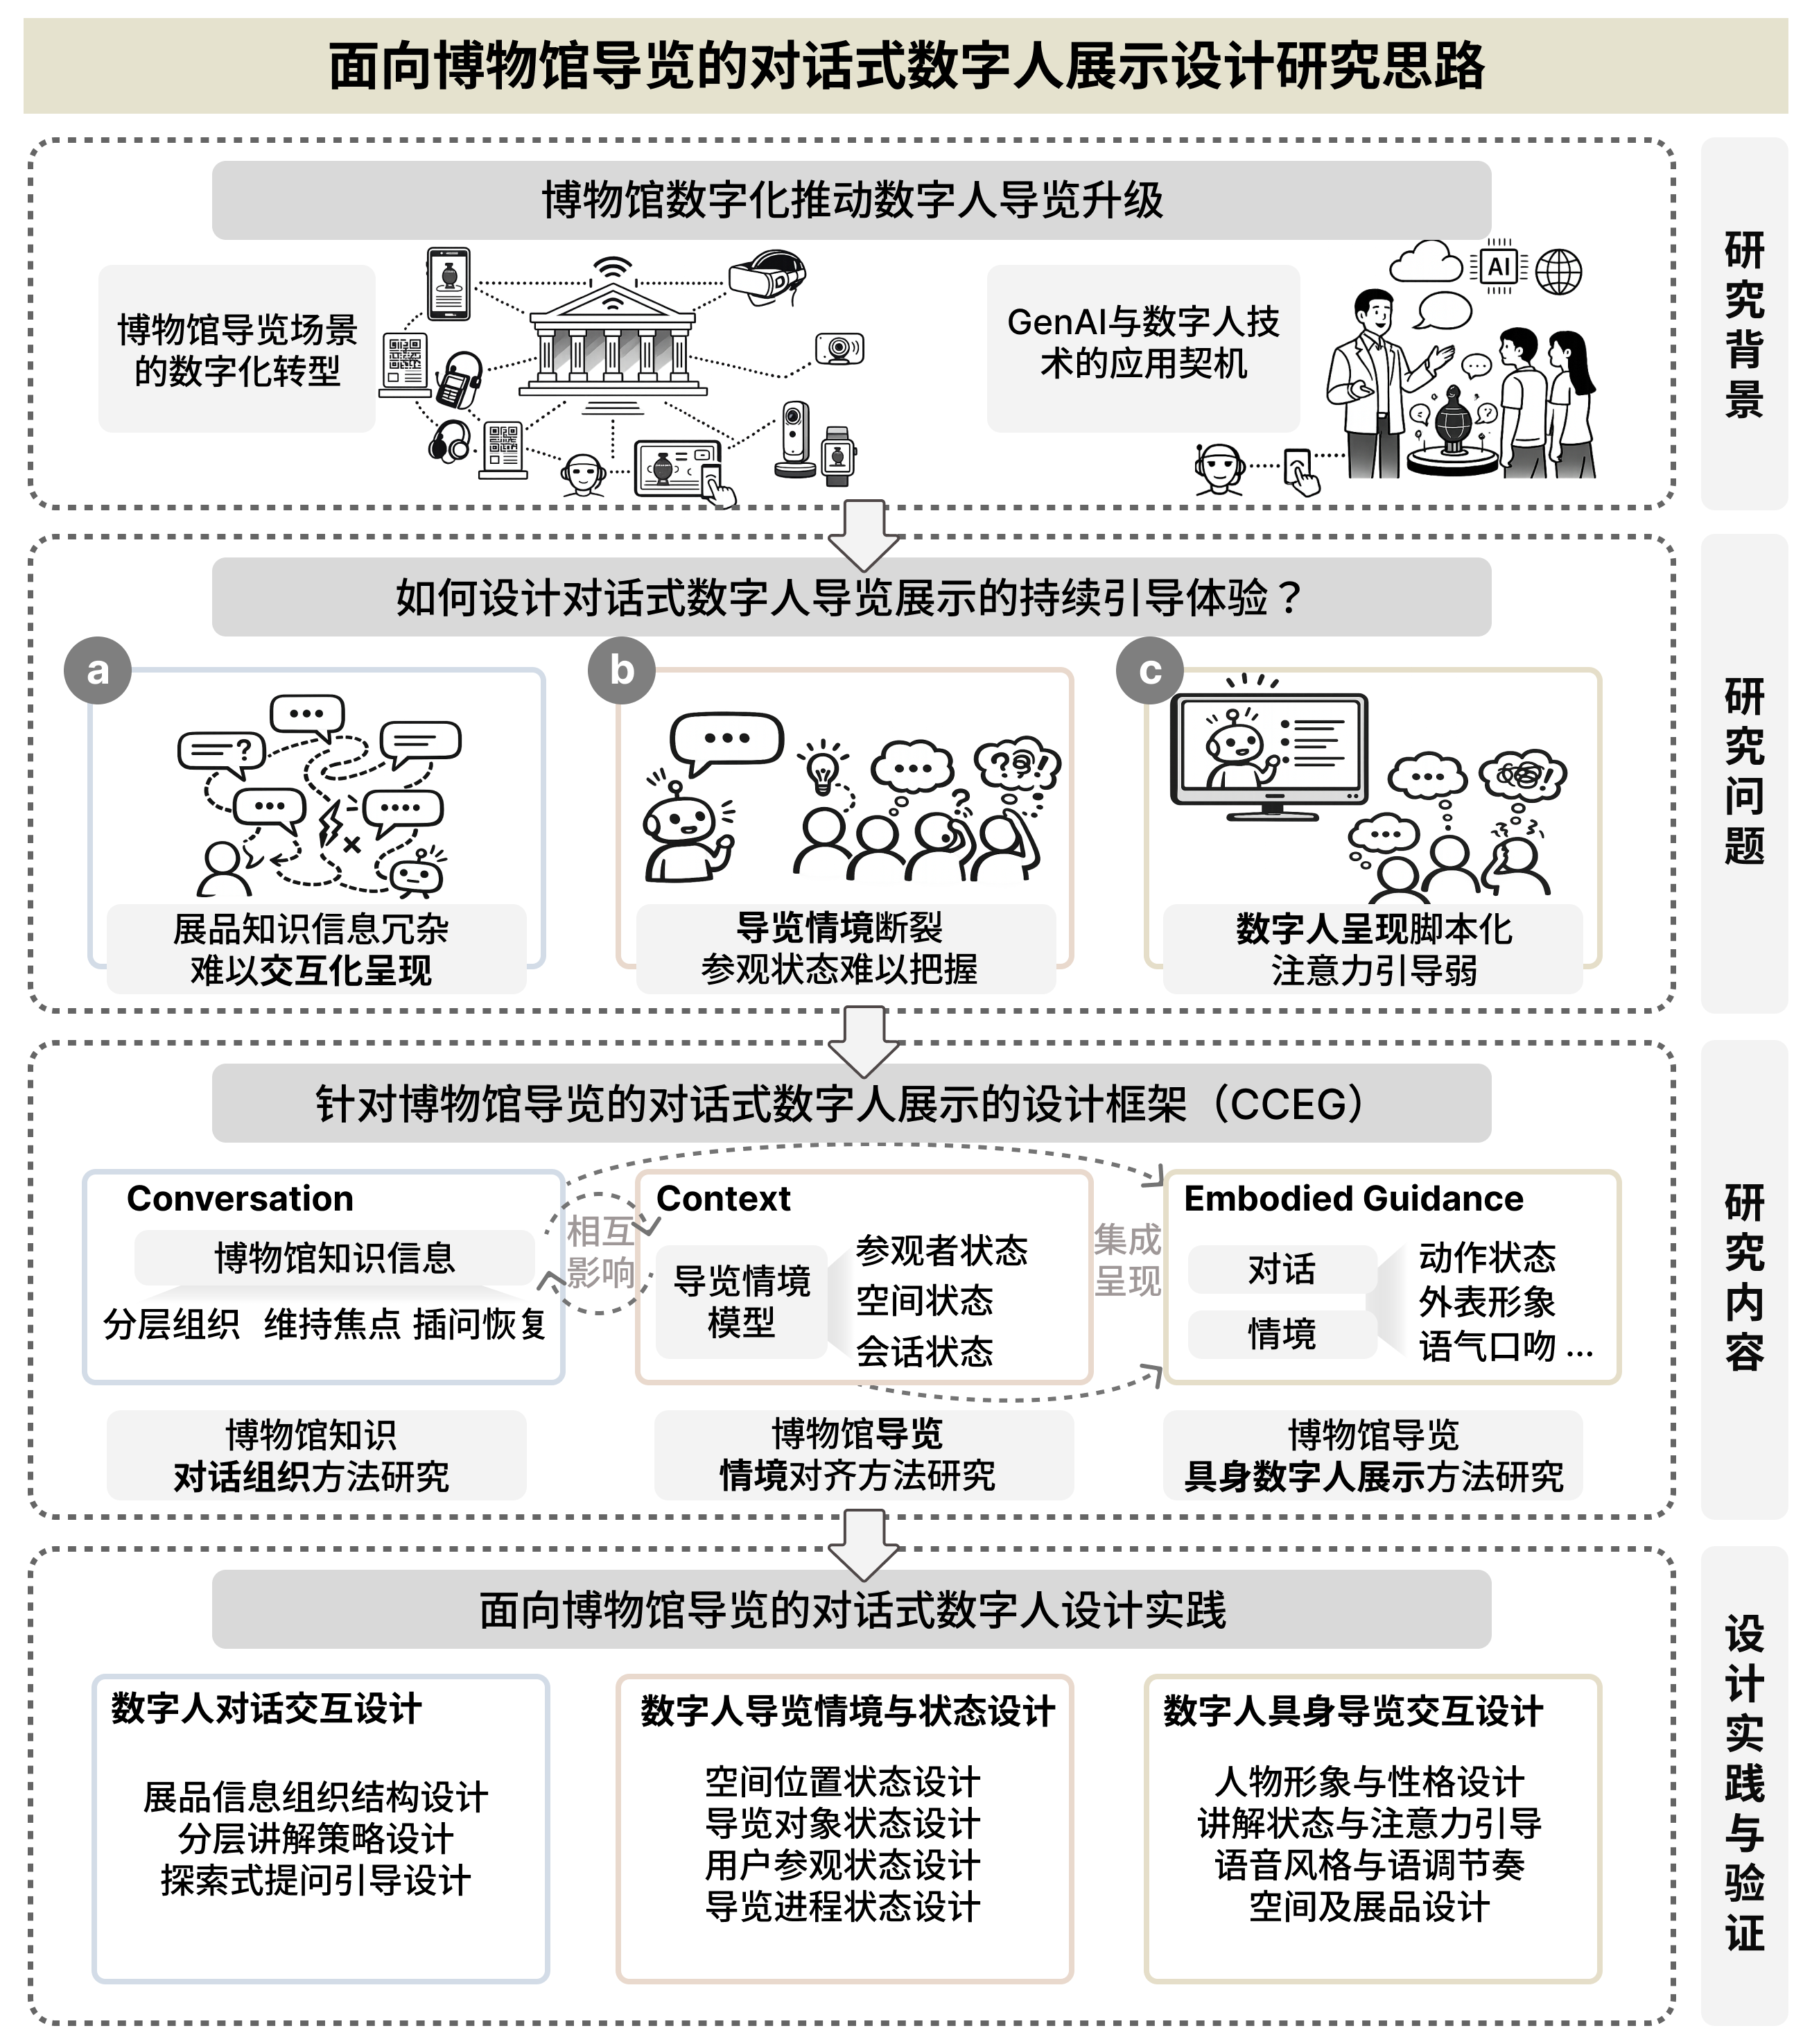
\includegraphics[width=\textwidth]{figure/figs/研究思路.png}
    \caption{本文的研究思路}
    \label{fig:research-roadmap}
\end{figure}

据此，本文将研究问题归纳为三个方面：
\begin{enumerate}[label=（\arabic*）]
\item 展品知识信息复杂，难以交互化呈现。现有相关展示常以固定脚本或单轮问答组织内容，难以形成分层解释、探索式提问引导与节奏化推进，导致观众获取到的是片段信息而非连续理解路径。
\item 导览情境易断裂，参观状态难以把握。观众在空间移动、对象切换与问题变化中不断重构关注点，相关展示若缺少可持续的情境建模与状态维护，便难以提供“此时此地”的导览响应。
\item 数字人呈现脚本化，注意力引导弱。现有数字人展示常停留在播报层，表达与语义、空间对象和引导意图不同步，难以形成可感知、可跟随的引导体验。
\end{enumerate}

针对上述问题，本文提出基于 CCEG 的研究内容框架：
\begin{enumerate}[label=（\arabic*）]
\item \textbf{Conversation：}围绕博物馆知识信息开展对话组织方法研究，构建分层解释、探索式提问引导与对话节奏机制，实现知识内容的可交互化呈现与持续推进。
\item \textbf{Context：}围绕导览情境对齐开展方法研究，建立导览情境模型，维护对话历史情境、交互语域情境与空间-展品情境，支持状态更新、内容选择与策略调节。
\item \textbf{Embodied Guidance：}围绕具身数字人展示开展方法研究，将对话与情境状态集成到动作、外表形象、语气口吻与行为编排中，提升引导的可感知性与可跟随性。
\end{enumerate}

在设计实践与验证层，本文进一步将上述框架落实为三类系统设计与实现：
\begin{enumerate}[label=（\arabic*）]
\item 数字人对话交互设计：包括展品知识库设计、分层讲解策略、探索式提问引导交互与对话节奏/转场规则。
\item 对话式数字人展示情境与状态设计：包括导览状态设计、状态更新策略、情境驱动内容选择与情境可视化调节。
\item 数字人具身导览交互设计：包括行为指向与引导、人物形象与性格设计、语音风格与语调节奏、注意力引导编排与空间/展品协同设计。
\end{enumerate}

\section{研究方法}
（1）系统性文献研究法

本文围绕博物馆学习、对话式交互、具身认知与对话式数字人展示四个主题，系统梳理国内外相关文献与研究报告，涵盖学术期刊、专著、会议论文与行业实践资料。通过对核心概念、研究范式与评价指标的归纳比较，明确本研究的问题边界、理论基础与关键变量，为 CCEG 框架建模提供可追溯的证据支撑。

（2）典型案例比较分析法

本文选取具有代表性的数字博物馆、文化遗产对话系统与虚拟导览代理案例，从知识组织方式、会话连贯机制、情境响应策略与多模态表达一致性等维度进行横向比较。除案例比较外，本文还开展了实地调研与问卷调查，并结合对观众与导览员的访谈结果进行综合分析。通过案例差异与共性特征分析，提炼可迁移的设计原则与失效模式，为框架细化与系统方案设计提供实践依据。

（3）跨学科综合研究法

本文整合设计学、叙事学、人机交互与人工智能相关方法，从“学习机制—交互机制—实现机制”三个层面建立统一分析视角。该方法用于打通理论论证与工程实现之间的断层，使导览目标、交互策略与技术模块能够在同一方法体系下被描述、验证与迭代。

（4）设计型研究与原型验证法

本文采用 Design Research 的路径，将理论结论转化为可运行的原型系统，并通过迭代开发验证设计假设。在验证阶段结合用户测试与过程数据分析，对理解度、参与度与引导感知等指标进行综合评估，检验所提框架与策略在真实导览任务中的有效性与可实施性。

\section{论文结构}
如图\ref{fig:thesis-structure}所示，本文在章节安排上围绕“背景研究—提出问题—分析问题—解决问题—设计实践—实验验证—总结展望”展开。

\begin{figure}[!htbp]
    \centering
    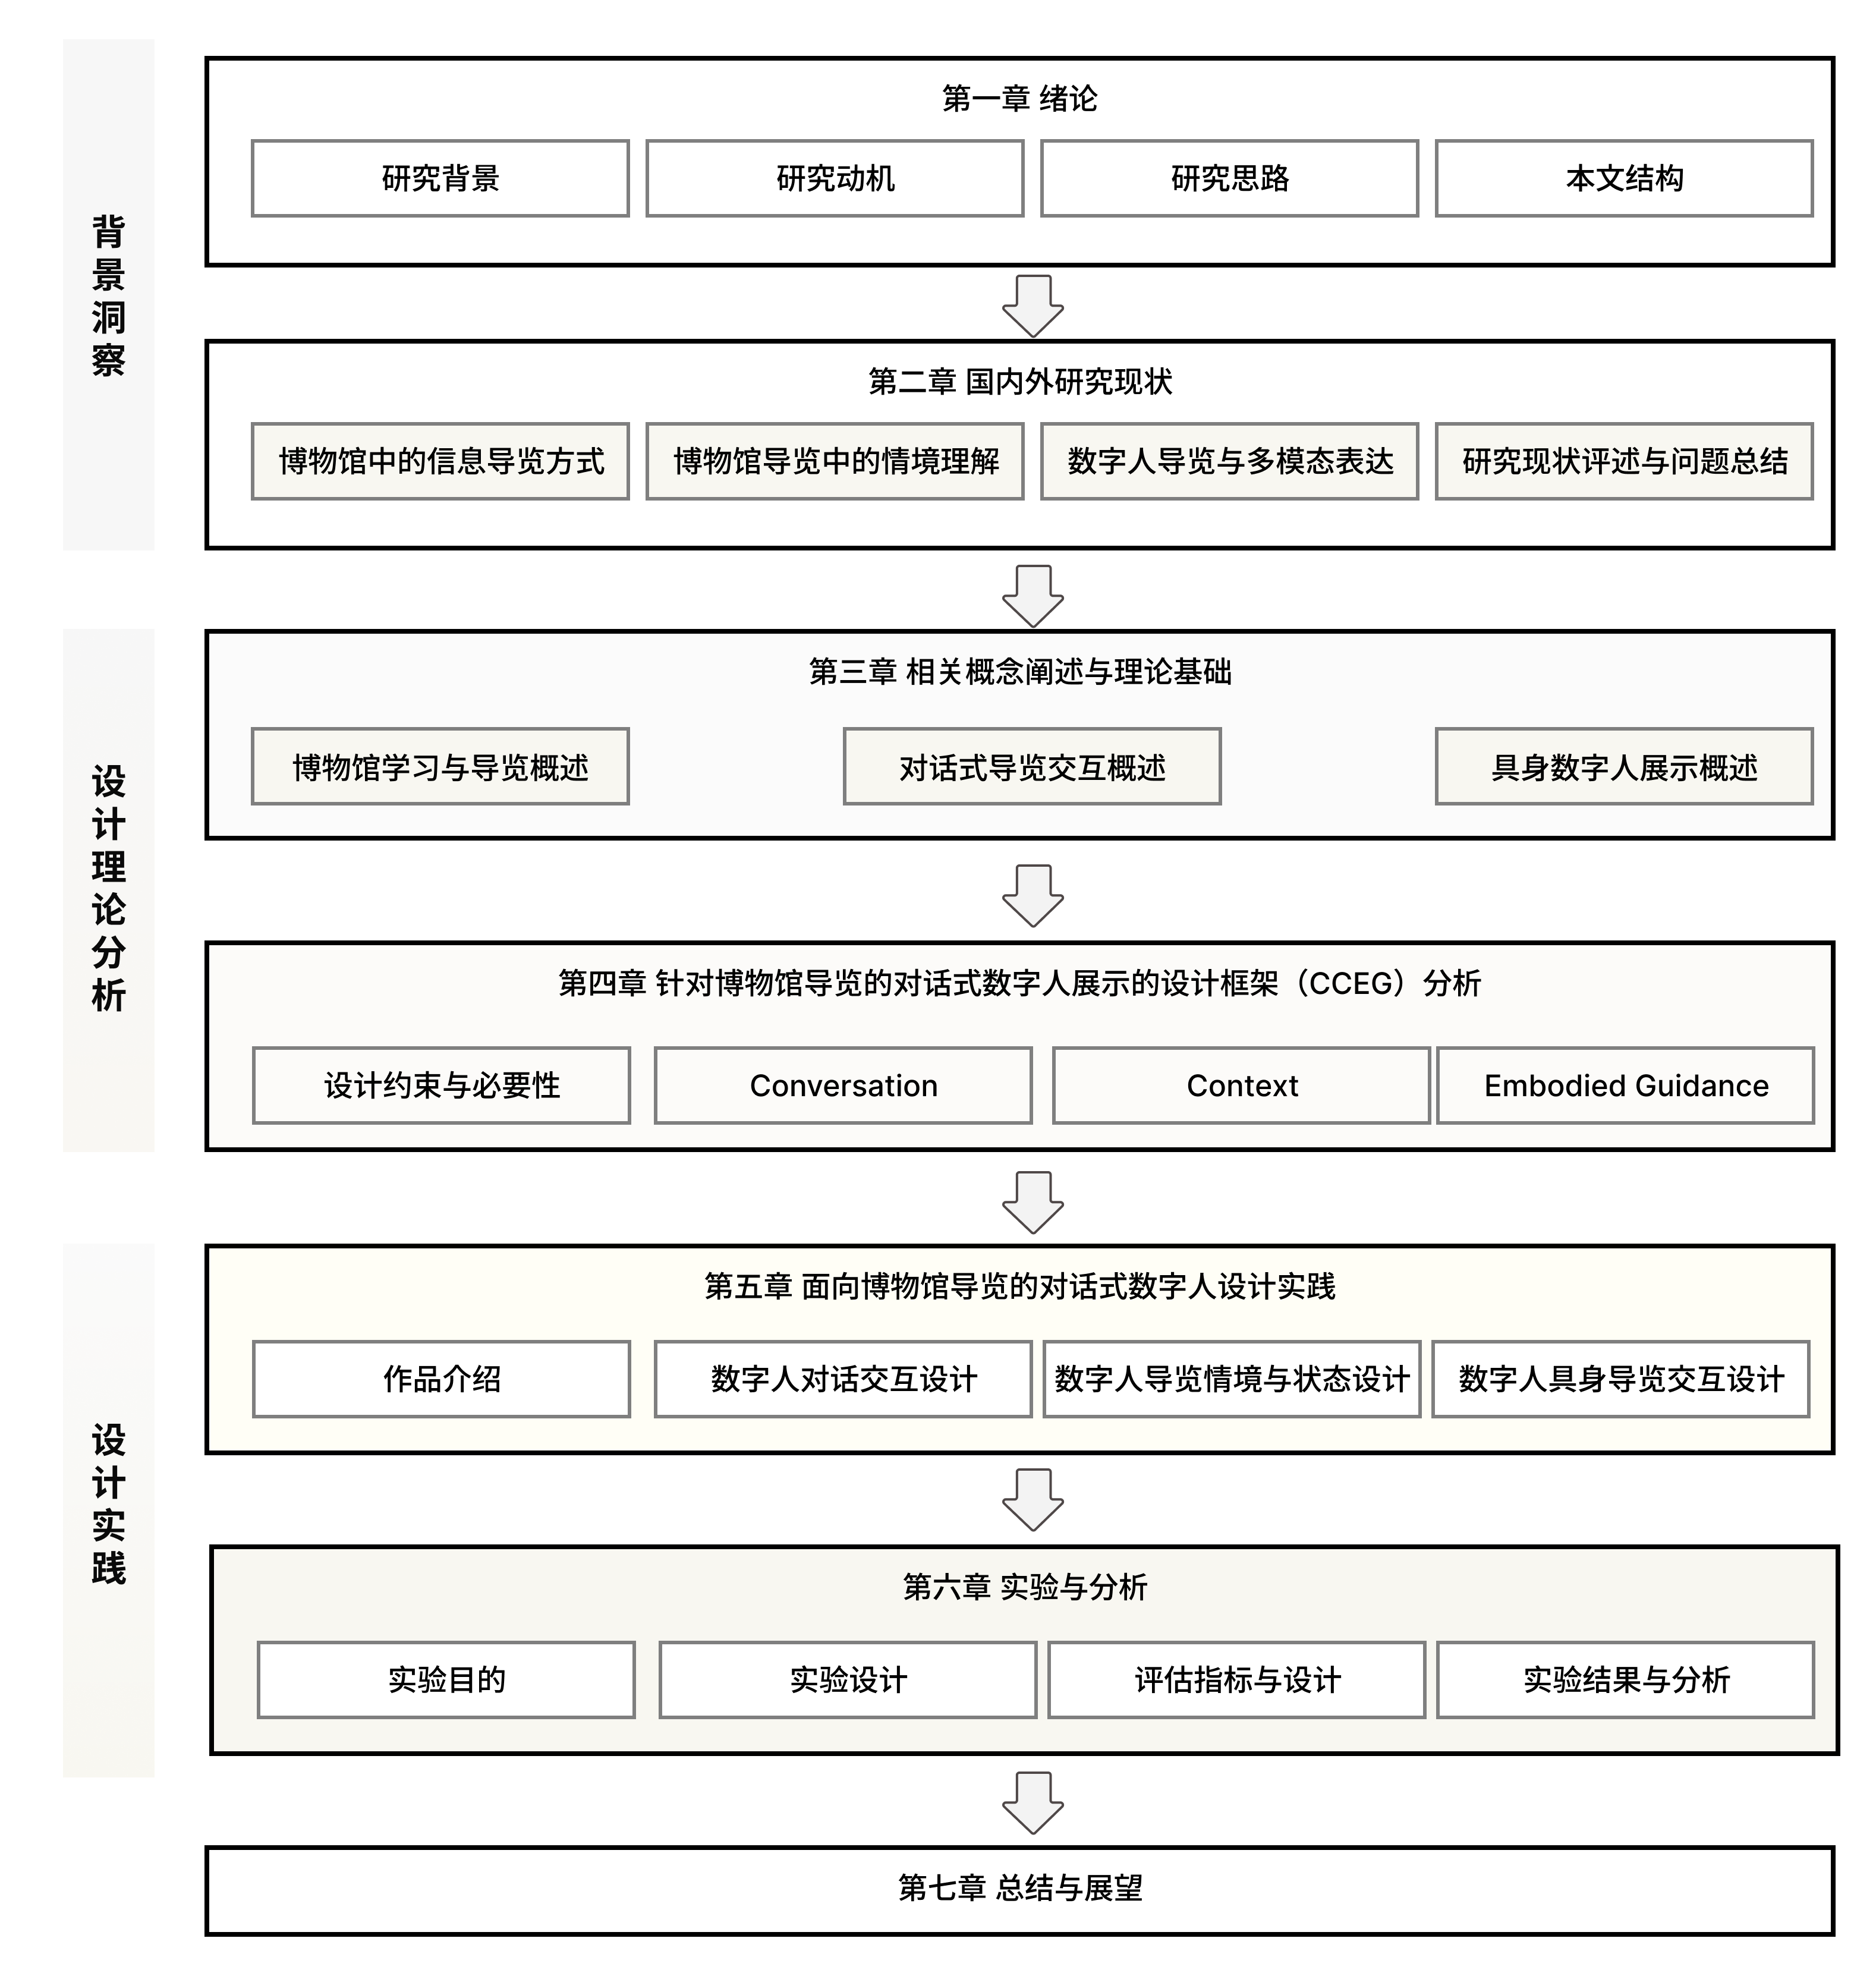
\includegraphics[width=\textwidth]{figure/figs/论文结构.png}
    \caption{本文的论文结构}
    \label{fig:thesis-structure}
\end{figure}

本文整体按照“背景研究—提出问题—分析问题—解决问题—设计实践—实验验证—总结展望”的链路展开。第一章为绪论，说明研究背景、研究动机、研究思路、研究方法、论文结构以及研究意义。第二章梳理国内外相关研究现状，并总结当前研究缺口与问题。第三章对博物馆学习、对话式导览交互与具身数字人展示等相关概念及理论基础进行阐述。第四章提出 CCEG 设计框架，并分别从 Conversation、Context 与 Embodied Guidance 三个维度展开分析。第五章基于该框架，进一步形成面向博物馆导览的对话式数字人展示设计实践方案。第六章通过实验与分析，对所提出设计方案的有效性进行验证。第七章对全文进行总结，并讨论研究不足与未来展望。

\section{研究意义与创新点}
（1）理论意义

本文从博物馆学习引导的设计视角切入，尝试厘清对话式数字人展示在导览场景中的组织逻辑与设计路径。一方面，本文系统梳理对话组织、导览情境与具身表达三类关键要素及其作用关系，明确对话式数字人展示从“信息播报”走向“学习引导”的理论转向；另一方面，结合 CCEG（Conversation--Context--Embodied Guidance）框架，构建出一套面向博物馆场景的结构化设计方法，以拓展现有数字导览与交互叙事研究在学习情境中的适用范围。

（2）实践意义

本文探索了对话式数字人展示设计在博物馆场景中的实际应用，并将理论成果转化为系统实践，基于原型系统验证该方法在真实交互中的可行性与有效性。本研究的实践成果不仅为对话式数字人展示设计与实现提供了可参考的落地路径，也为公共文化传播、展览教育服务与数字内容体验设计提供了可迁移的方法启示，进一步拓展相关应用场景的创新可能性。

（3）创新点

本文在设计研究范式下形成“框架提出—系统实现—实证验证”的一体化研究路径，主要体现在以下三个方面。

第一，交互框架方面。本文提出 CCEG（Conversation--Context--Embodied Guidance）导览设计框架，将导览对话组织、参观情境维持与具身表达协同纳入同一交互模型，明确对话式数字人展示从“能回答”到“能引导”的设计逻辑。

第二，交互策略方面。本文围绕博物馆导览任务提出分层讲解、探索式提问引导推进、导览阶段切换与注意力引导等策略，并将其映射为可执行的状态驱动机制，使数字人在真实参观过程中能够根据观众问题与场景变化动态调整交互方式。

第三，交互评估方面。本文将对话式数字人展示交互效果评估扩展为“理解度—参与度—引导感知”三维联合评估，并结合用户实验、过程数据与主观反馈进行综合验证，为博物馆数字人交互设计提供可参考的评估路径与证据支撑。
